\documentclass[a4paper,12pt]{scrartcl}

\usepackage[utf8]{inputenc}
\usepackage[ngerman]{babel}
\usepackage{amsmath}
\usepackage[a4paper, left=3cm, right=2.5cm, top=2.5cm, bottom=3cm]{geometry}
\usepackage{graphicx}
\usepackage{csquotes}
\usepackage{hyperref}
\usepackage[figure]{hypcap}
\usepackage{listings}
\usepackage{xcolor}

\definecolor{codegreen}{rgb}{0,0.6,0}
\definecolor{codegray}{rgb}{0.5,0.5,0.5}
\definecolor{codepurple}{rgb}{0.58,0,0.82}
\definecolor{backcolour}{rgb}{0.95,0.95,0.92}

\lstdefinestyle{mystyle}{
    backgroundcolor=\color{backcolour},   
    commentstyle=\color{codegreen},
    keywordstyle=\color{magenta},
    numberstyle=\tiny\color{codegray},
    stringstyle=\color{codepurple},
    basicstyle=\ttfamily\footnotesize,
    breakatwhitespace=false,         
    breaklines=true,                 
    captionpos=b,                    
    keepspaces=true,                 
    numbers=left,                    
    numbersep=10pt,                  
    showspaces=false,                
    showstringspaces=false,
    showtabs=false,                  
    tabsize=2,
    language=Python
}

\lstset{style=mystyle}

\usepackage{footnote}
\makesavenoteenv{table}
\makesavenoteenv{tabular}

\title {\textbf{Ausarbeitung}}
\author{Zoe Luca Günther}

\makeatletter
\def\@maketitle{%
  \newpage
  \null
  \vskip 15em%
  \begin{center}%
  \let \footnote \thanks
    {\LARGE \@title \par}%
    \vskip 1em%
    {\Large Ein Snake Spiel mit Darstellung über einen Raspberry Pi \par}%
    \vskip 5em%
    {\large
      \lineskip .5em%
      \begin{tabular}[t]{c}%
        \@author
      \end{tabular}\par}%
    \vskip 1em%
    {\large \@date}%
  \end{center}%
  \par
  \vskip 1.5em}
\makeatother

\begin{document}

\pagenumbering{Roman}
\maketitle
\newpage
\tableofcontents
\newpage
\listoffigures
\newpage
\pagenumbering{arabic}

\section{Einleitung}
%%%%%%%%%%%%%%%%%%%%%%%%%%%%%%%%%%%%%%%%%%%%%%%%%%%%
%	Einleitung
%%%%%%%%%%%%%%%%%%%%%%%%%%%%%%%%%%%%%%%%%%%%%%%%%%%%

In diesem Projekt habe ich ein Snake Spiel entwickelt. Hierbei ist das besondere, dass man dieses Snake Spiel über die Lagesensoren des Handys steuern kann. Man verbindet sich mit einer Website, geht in die Warteschlange rein und sobald man an der Reihe ist, wird man zur Spielsteuerung weitergeleitet [\ref{fig:main-menu}][\ref{fig:main-menu-queue}]. Am Anfang jedes Spiels wird ein kurzer Hinweis am Handy eingeblendet, welcher einem sagt, dass man das Handy vertikal und flach halten soll und die Bildschirmrotation deaktiviert werden sollte [\ref{fig:controller-hint-1}][\ref{fig:controller-hint-2}]. Dies ist wichtig, damit die Steuerung richtig funktioniert, da man um das Spiel zu steuern, lediglich sein Handy neigen muss. Um Das Spielerlebnis so gut wie möglich zu halten, muss das Handy flach und vertikal gehalten werden, da so die Steuerung am besten funktioniert, da diese sehr sensibel sein kann.
Um das Spielgeschehen zu sehen, wird ein Raspberry Pi mit einer 64x64 LED Matrix verwendet, worauf der Score und das Spiel dargestellt werden. Um das Spiel zu pausieren, klickt man lediglich auf seinem Handy auf den Pause Button [\ref{fig:controller}]. Dies geht jedoch nur, wenn man gerade an der Reihe ist. Um dies zu überprüfen, wird beim ersten betreten der Spiel Website ein Cookie gesetzt, worin die User ID steht. Jede ID ist unterschiedlich, um eine genaue Identifizierung zu ermöglichen.
Sollte sich ein Spieler für mehr als 20 Sekunden im Pause Status befinden, oder mehr als 20 Sekunden keine Bewegung mehr machen, wird das Spiel beendet und der nächste Spieler aus der Warteschlange kann spielen. Nachdem man sich selber als Schlange gefressen hat, oder man zu lange im Spiel war, wird man auf eine Game Over Seite weitergeleitet, wo der eigene Score eingeblendet wird [\ref{fig:gameover}].
% bilder als anhang

\section{Vorgehensweise}
%%%%%%%%%%%%%%%%%%%%%%%%%%%%%%%%%%%%%%%%%%%%%%%%%%%%
%	Vorgehensweise
%%%%%%%%%%%%%%%%%%%%%%%%%%%%%%%%%%%%%%%%%%%%%%%%%%%%

% wie bin ich vorgegangen und welche tools habe ich benutzt
% erst in pygame das grundgerüst gemacht
% dann die api
% dann die darstellung auf dem raspi mit rpi rgb matrix api
% welche bibliothekene habe ich benutzt
% warum lagesensor

Das Projekt wurde in verschiedene Unterpunkte eingeteilt, um die bestmögliche Implementierung sicherzustellen.


\subsection{Grundgerüst}
%%%%%%%%%%%%%%%%%%%%%%%%%%%%%%%%%%%%%%%%%%%%%%%%%%%%
%	Grundgerüst
%%%%%%%%%%%%%%%%%%%%%%%%%%%%%%%%%%%%%%%%%%%%%%%%%%%%
\label{grundgerüst}
Das Grundgerüst besteht aus verschiedenen Klassen, welche für den Spielablauf essentiell sind. Folgende Klassen beinhaltet das Grundgerüst:

\newpage

\begin{table}
\centering
\begin{tabular}[!htb]{p{4cm}|p{10cm}}
Klassenname & Beschreibung \\
\hline
Player.py & Zuständig für die Bewegung des Spielers, des Überprüfens auf Kollision, das Score Handling und das Fressen von Futter \\
Logger.py & Ausgeben von Nachrichten in der Konsole zu Debug Zwecken. Es kann ein Prefix der Klasse Prefix.py angegeben werden \\
Playground.py & Handling des Spielfeld, setzen von Blöcken\footnote{Das Spielfeld besteht aus Blöcken, welche in einem 2d Array gespeichert sind} auf dem Spielfeld, setzen einer Random Futter Position, Prüfen ob das Spielfeld voll ist \\
Queue.py & Generelles Queue Handling (Spieler hinzufügen, entfernen aus Queue), Nächsten Spieler nehmen, UserId verifizieren\footnote{Überprüfen ob die UserId die nötige länge hat} \\
SnakeGame.py & Game Status setzen, Game starten / stoppen / pausieren, Game loop, game resetten, game over Handling \\
\end{tabular}
\caption{Grundgerüst Klassen}
\end{table}

\begin{table}
\centering
\begin{tabular}[!htb]{p{4cm}|p{10cm}}
Klassenname & Beschreibung \\
\hline
Direction.py & Richtungsangaben \\
GameStatus.py & Gamestatus mit Gamestatus Text \\
Message.py & Game over Nachrichten \\
PlaygroundTile.py & Spielfeld Blöcke (zum Beispiel Wand, Snake, Futter) \\
Prefix.py & Prefix zu Debug Zwecken \\
\end{tabular}
\caption{Enum Klassen}
\end{table}

Zum testen der Funktionalitäten, wurde das Spiel vorerst mithilfe der Bibliothek \textit{pygame} implementiert. Somit konnte das Spiel dargestellt werden, die Bewegungsabläufe getestet und der Spielablauf angepasst werden. Für den Gameloop wurde jedoch zu diesem Zeitpunkt die pygame eigenen Funktionen verwendet. Die Steuerung wurde vorerst über die Tastatur implementiert, da die spätere Steuerung über die Website mithilfe der API Schnittstelle funktioniert.

\subsection{Website}
%%%%%%%%%%%%%%%%%%%%%%%%%%%%%%%%%%%%%%%%%%%%%%%%%%%%
%	Website
%%%%%%%%%%%%%%%%%%%%%%%%%%%%%%%%%%%%%%%%%%%%%%%%%%%%
Der Hauptteil der Website besteht aus dem Styling (CSS\footnote{Cascading Style Sheets, Gestaltungs- und Formatierungssprache}) und den Funktionen (JS\footnote{JavaScript, für dynamisches HTML}), da im Hintergrund auf die API Schnittstelle zugegriffen werden muss und um Animationen für den Benutzer anzuzeigen, um das Benutzererlebnis an erster Stelle zu halten. Somit ist die Website speziell für die Mobilen Endgeräte konzipiert, da die Steuerung über dieses im weiteren Verlauf erfolgt. Was diese Spezialisierung ausmacht ist, dass die Schriftgröße besonders auf kleine Geräte angepasst ist und die Ladezeiten so gering wie möglich gehalten werden, da diese Seite meist aus dem normalen Mobilfunknetz aufgerufen wird. Außerdem wird ein responsive Design\footnote{Responsive bedeutet in dem Fall zum Beispiel ``auf jemanden eingehen'' oder ``reaktionsfähig bleiben''} verwendet, um die Website jederzeit an fast jedes Endgerät anzupassen. ``Mobile first'' spielt hierbei eine große Rolle, unter dem Aspekt der Steuerung, aber auch unter dem Aspekt, dass man davon ausgehen kann, dass die meisten Websites heutzutage mit dem Smartphone aufgerufen werden, da man dies zu jederzeit dabei haben kann. \\
Die Website besteht aus drei HTML Seiten:

\begin{table}
\centering
\begin{tabular}[!htb]{p{4cm}|p{4cm}|p{8cm}}
Dateiname & Beschreibung \\
\hline
index.html & ``Startseite'' der Website. Joinen der Queue \\
controller.html & Steuerung der Snake \\
gameover.html & Game over Screen nach beenden des Spiels. \\
\end{tabular}
\caption{HTML Dateien}
\end{table}

Um die Funktionalität der Website zu gewährleisten, wird wie oben erwähnt, JS verwendet. Hierfür wird jeder HTML Datei eine JS Datei zugewiesen:


\begin{table}
\centering
\begin{tabular}[!htb]{p{4cm}|p{4cm}|p{8cm}}
Dateiname & Beschreibung \\
\hline
controller.js & Funktionalität und anzeige der Steuerung. Starten und pausieren des Spiels \\
gameover.js & Laden und anzeigen des Scores. \\
index.js & Anzeigen der aktuellen Spieler in der Warteschlange. Betreten und verlassen der Warteschlange. Anzeigen der Warteschlangen Animation. \\
constants.js & Konstante Variablen für die API Schnittstelle. \\
\end{tabular}
\caption{JS Dateien}
\end{table}

Hierbei ist zu beachten, dass die Konstanten Variablen in jeder HTML Datei eingebunden sind, um jederzeit Zugriff auf die API Schnittstelle zu bekommen. Hinzu kommen Klassen, welche als Handler dienen:

\newpage
\begin{table}
\centering
\begin{tabular}[!htb]{p{4cm}|p{4cm}|p{8cm}}
Dateiname \\
\hline
controller\_handler.js \\
cookie\_handler.js \\
queue\_handler.js \\
score\_handler.js \\
\end{tabular}
\caption{Handler Klassen}
\end{table}

Diese Klassen beinhalten alle nötigen Funktionen, um auf die API Schnittstelle zuzugreifen und die dadurch entstandenen Daten zurückzugeben, um das handling in den jeweiligen Klassen zu vereinfachen. Es ist zu beachten, dass Funktionen teilweise Asynchron sind, was daran liegt, dass Daten, welche zur weiteren Verarbeitung benötigt werden (zum Beispiel zur Darstellung), erst zurückgegeben werden können, wenn diese vorliegen. Somit werden diese Funktionen in einem Promise gehandhabt. Die API Zugriffe werden über einen Standard fetch Aufruf gehandhabt. \\
Um das Benutzererlebnis zu verbessern, werden beim Game over Animationen angezeigt, welche den Score darstellen. Somit kann damit ein positives Erlebnis verbunden werden.


\subsection{API Schnittstelle}
%%%%%%%%%%%%%%%%%%%%%%%%%%%%%%%%%%%%%%%%%%%%%%%%%%%%
%	API Schnittstellt
%%%%%%%%%%%%%%%%%%%%%%%%%%%%%%%%%%%%%%%%%%%%%%%%%%%%

Das Web Framework \textit{fastapi} ist ein modernes, hoch performanted Python Framework. Es ist einfach zu handhaben und bietet alle nötigen Funktionen, welche in diesem Projekt benötigt werden. Diese sind verschiedene CRUD\footnote{create, read, update, delete} Operationen, das mitgeben eines HTML Statuscodes und das auslesen von Cookies, um die UserId abzufragen. Um die verschiedenen Klassen aus \autoref{grundgerüst} zu verwenden, muss dem Systempfad ein weiterer Pfad hinzugefügt werden, dem Übergeordneten Ordner, da sich die Backend API in einem eigenen Unterordner befindet:

\begin{lstlisting}
import sys

sys.path.append('../snake')

"""
Ordnerstruktur:

snake
	backend
	static
	enums
"""
\end{lstlisting}

Jede Schnittstelle hat anfangs den gleichen Ablauf: Es wird überprüft, ob ein UserId Cookie vorhanden ist. Ist dies nicht der Fall, wird durch den Logger, welcher in \autoref{grundgerüst} beschrieben ist, eine Mitteilung ausgegeben und der weitere Zugriff verwährt. Es wird ein JSON Objekt zurückgegeben, welches eine Nachricht und den Erfolgsstatus beinhaltet. Der Statuscode wird hierbei auf \textit{401 UNAUTHORIZED} gesetzt:

\begin{lstlisting}
if not userId:
	Logger.log(f"{userId}: UNAUTHORIZED", Prefix.API)
	response.status_code = status.HTTP_401_UNAUTHORIZED
	return {"message": "userId cookie not set", "success": False}
\end{lstlisting}

Sind die weiteren Voraussetzungen erfüllt, wie in etwa ob der Spieler, welcher eine Bewegung angefragt hat momentan an der Reihe ist, wird die jeweilige Aktion ausgeführt und der Benutzer, welcher die Anfrage gestellt hat, bekommt eine Erfolgsmeldung:

\begin{lstlisting}
return {"message": f"success message", "success": True}
\end{lstlisting}

Die JSON Objekte werden im Frontend verarbeitet.\\
Folgende Operationen werden durch die API geboten:


\newpage

\begin{table}
\centering
\begin{tabular}[!htb]{p{4cm}|p{4cm}|p{8cm}}
Pfad & REST (CRUD Operation) & Beschreibung \\
\hline
/move/{direction} & Put (update) & Bewegt die Snake in eine neue Richtung \\
/start & Put (create) & Startet das Spiel \\
/pause & Put (update) & Pausiert das Spiel \\
/queue/join & Put (create) & Tritt der Queue bei \\
/queue/leave & Put (update) & Verlässt die Queue \\
/queue/length & Get (read) & Fragt die aktuelle Queue größe ab. Wenn ein Spieler momentan spielt, zählt dieser als ein Spieler in der Queue extra \\
/current\_user & Get (read) & Fragt ab, ob der Spieler, welcher die Anfrage gestellt hat, berechtigt ist zu Spielen (als nächstes dran ist) \\
/surrender & Delete (delete) & Gibt das Spiel direkt auf (für Debug Zwecke) \\
/gameover & Get (read) & Gibt zurück ob das Spiel vorbei ist und ob der Benutzer momentan Berechtigt ist zu spielen \\
/score & Get (read) & Gibt den Score zurück, sofern der Spieler bereits ein Spiel gespielt hat \\
/threads & Get (read) & Gibt alle laufenden Threads aus (für Debug Zwecke)
\end{tabular}
\caption{API Methoden}
\end{table}

% Uvicorn mit einbringen

\subsection{Darstellung}
%%%%%%%%%%%%%%%%%%%%%%%%%%%%%%%%%%%%%%%%%%%%%%%%%%%%
%	Darstellung
%%%%%%%%%%%%%%%%%%%%%%%%%%%%%%%%%%%%%%%%%%%%%%%%%%%%

Für die Darstellung des Spielfeldes und des Scores wird die Bibliothek \textit{rpi-rgb-led-matrix} verwendet. Diese Bibliothek ist auf https://github.com/hzeller/rpi-rgb-led-matrix zu finden. Sie wird direkt auf dem Raspberry Pi installiert und kann direkt in Python eingebunden werden. Dank dieser Bibliothek kann man einzelne Pixel darstellen, oder ganze Texte. Es werden verschiedene Schriftgrößen mitgeliefert. Um das Spielfeld darzustellen, wird die Spielfeldmatrix genommen und in Pixel übersetzt. Jeder Spielfeldblock wird auf der LED Matrix in der Größe 2x2 dargestellt, um die Sichtbarkeit zu erhöhen. Außerdem wurde der Hintergrund dunkler eingestellt von der Helligkeit her, um das Spielerlebnis zu fördern. Die Display Klasse, welche für die Darstellung zuständig ist, ist von der Klasse \textit{SampleBase.py} abgeleitet und beinhaltet daher die Funktion \textit{process}, welche den infinity loop und somit die Darstellung startet. Die Display Klasse beinhaltet daher eine Funktion \textit{terminate}, um den loop zu unterbrechen. Die damit verbundenen Schwierigkeiten sind in \autoref{schwierigkeiten} beschrieben.


\label{schwierigkeiten} % schwierigkeit mit reinbringen, dass uvicorn gestartet werden musste über startbefehl außerhalb der console
\section{Schwierigkeiten}
%%%%%%%%%%%%%%%%%%%%%%%%%%%%%%%%%%%%%%%%%%%%%%%%%%%%
%	Schwierigkeiten
%%%%%%%%%%%%%%%%%%%%%%%%%%%%%%%%%%%%%%%%%%%%%%%%%%%%

Die größte Schwierigkeit war, die API nicht zu unterbrechen, während das Spiel läuft. Es wurde \textit{multithreading} verwendet, um verschiedene Thread parallel laufen zu lassen. Somit laufen im fertigen Projekt der Thread für die Darstellung des Spiels auf dem Raspberry Pi, der Gameloop, die Überprüfung ob ein Spieler keine Inputs mehr macht und somit nicht mehr anwesend ist (AFK\footnote{away from keyboard, abwesend}) und die API Schnittstelle parallel. Es wurde versucht, einen neuen Prozess für die Darstellung auf dem Display zu verwenden, jedoch können live updates in einem separaten Prozess nicht mehr nachverfolgt werden, weshalb die Thread Variante verwendet worden ist. Die Thread wurden als \textit{daemon} Threads gestartet, damit man sie zu jedem Zeitpunkt durch ein Interrupt unterbrechen kann. Die Implementierung sieht wie folgt aus, sobald die start Methode von der API Schnittstelle aufgerufen wird:

% hier code von den threads anzeigen.
\begin{lstlisting}
import threading

# Threads initialisieren
displayThread = threading.Thread(name="Display", target=display.process)
displayThread.daemon = True

gameLoopThread = threading.Thread(name="Gameloop", target=self.loop)
gameLoopThread.daemon = True

gameLoopAfkThread = threading.Thread(name="GameloopAfk", target=self.loopAfkCheck)
gameLoopAfkThread.daemon = True
        
# Threads starten
gameLoopThread.start()
displayThread.start()
gameLoopAfkThread.start()

# Threads beenden
gameLoopThread.join()
self.loopAfkCheckRunning = False
gameLoopAfkThread.join()
display.terminate()
displayThread.join()
\end{lstlisting}

Entscheidend ist hierbei die Reihenfolge, in der die Threads gestartet und gestoppt werden. Zu beachten ist außerdem, dass der Display Thread eine Funktion benötigt, um terminiert zu werden, ansonsten kann er nicht gestoppt werden. die Loops greifen jeweils auf den Gamestatus zu, um den in jedem Thread integrierten \textit{infinity loop} zu unterbrechen, sollte sich der Gamestatus ändern und der Thread nicht mehr benötigt werden. Somit erklärt sich auch die Reihenfolge, in welcher die Thread beendet werden. Sobald das Spiel vorbei ist und der Gameloop beendet wird, kann die afk Überprüfung ebenfalls beendet werden. Da das Spiel vorbei ist wird außerdem zum Schluss der Displaythread beendet, da es kein Spiel mehr zum darstellen gibt. Somit gehen alle Aktionen der restlichen Threads vom eigentlichen Gameloop aus.

\section{Ergebnisse}
%%%%%%%%%%%%%%%%%%%%%%%%%%%%%%%%%%%%%%%%%%%%%%%%%%%%
%	Ergebnisse
%%%%%%%%%%%%%%%%%%%%%%%%%%%%%%%%%%%%%%%%%%%%%%%%%%%%

\newpage
\section{Abbildungen}
%%%%%%%%%%%%%%%%%%%%%%%%%%%%%%%%%%%%%%%%%%%%%%%%%%%%
%	Abbildungen
%%%%%%%%%%%%%%%%%%%%%%%%%%%%%%%%%%%%%%%%%%%%%%%%%%%%

% hauptmenü
\begin{figure}[!h]
   \begin{minipage}[t]{.4\linewidth}
      \includegraphics[width=\linewidth]{Abbildungen/Snake_Hauptmenü.png}
      \caption{Snake Website Hauptmenü}
      \label{fig:main-menu}
   \end{minipage}
   \hspace{.1\linewidth}% Abstand zwischen Bilder
   \begin{minipage}[t]{.4\linewidth}
      \includegraphics[width=\linewidth]{Abbildungen/Snake_Hauptmenü_Warteschlange.png}
      \caption{Snake Website Hauptmenü in Warteschlange}
      \label{fig:main-menu-queue}
   \end{minipage}
\end{figure}

\newpage

% hints
\begin{figure}[!h]
   \begin{minipage}[t]{.4\linewidth}
      
\includegraphics[width=\linewidth]{Abbildungen/Snake_Controller_hint_1.png}
      \caption{Snake Website Controller Hinweis 1}
      \label{fig:controller-hint-1}
   \end{minipage}
   \hspace{.1\linewidth}% Abstand zwischen Bilder
   \begin{minipage}[t]{.4\linewidth}
      
\includegraphics[width=\linewidth]{Abbildungen/Snake_Controller_hint_2.png}
      \caption{Snake Website Controller Hinweis 2}
      \label{fig:controller-hint-2}
   \end{minipage}
\end{figure}

\newpage

% controller und gameover
\begin{figure}[!h]
   \begin{minipage}[t]{.4\linewidth}
      
\includegraphics[width=\linewidth]{Abbildungen/Snake_Controller.png}
      \caption{Snake Website Controller}
      \label{fig:controller}
   \end{minipage}
   \hspace{.1\linewidth}% Abstand zwischen Bilder
   \begin{minipage}[t]{.4\linewidth}
      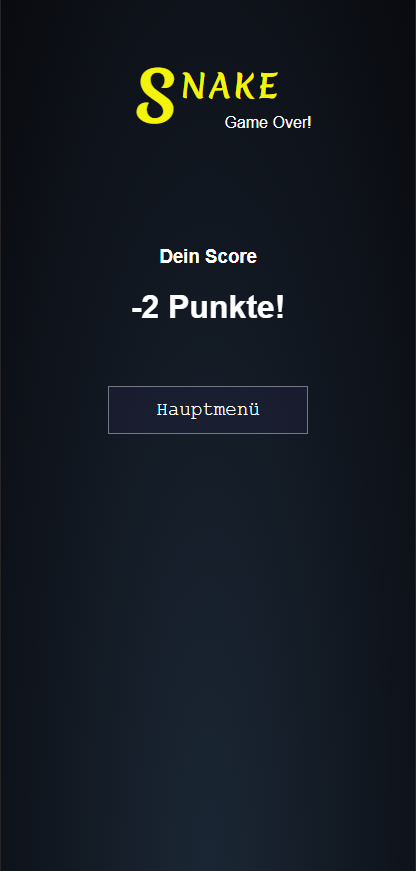
\includegraphics[width=\linewidth]{Abbildungen/Snake_Gameover.png}
      \caption{Snake Website Game Over Score}
      \label{fig:gameover}
   \end{minipage}
\end{figure}

\newpage

\section{Quellenverzeichnis}
%%%%%%%%%%%%%%%%%%%%%%%%%%%%%%%%%%%%%%%%%%%%%%%%%%%%
%	Quellenverzeichnis
%%%%%%%%%%%%%%%%%%%%%%%%%%%%%%%%%%%%%%%%%%%%%%%%%%%%

\begin{itemize}
\item \url{https://www.konversionskraft.de/trends/die-3-saeulen-des-responsive-webdesign.html} \\ Stand: 16.08.2022
\item \url {https://tetris.informatik.fh-swf.de/snake/index.html} \\ Stand: 16.08.2022
\end{itemize}

\end{document}